\documentclass[../main/main.tex]{subfiles}

% Put everything that shall appear in the discussion
% inside this document environment.
\begin{document}
	
	\noindent Our goal was to design and evaluate an experiment which measures how well people estimate their performance. We created a questionnaire, where subjects had to solve eight sorting tasks. The questionnaire had two conditions: sorting without and with active recall. When sorting without active recall, we provided the answers to the task in a randomized order. The subjects simply needed to bring the given items into the correct order. When sorting with active recall, we did not provide any hints to the solution. The subjects had to actively recall the items in question and bring them into the correct order. In total we collected seven tasks for condition one and one task for condition two. After finishing a task, the subjects had to estimate their performance by drawing a probability density function. 
	
	After collecting the answers from fourteen subjects, our program read the probability density functions, extracted the probabilities at discrete points and normalized these probabilities. Additionally, the program scored the answers of each subject for each task. Then we used these two quantities to calculate the Brier score, a score to measure the accuracy of probabilistic predictions, for each participant and each task.
	
	Unfortunately, the active recall item of condition two turned out to be inappropriate for determining the accuracy of performance self-evaluation, which is why we excluded it from the main part of our evaluations (for more detail see next section).
	\\\\
	In sections \ref{sec:finding_task_type} to \ref{sec:explaining_pdf} we discuss the creation and design of the questionnaire. We review different task types (\ref{sec:finding_task_type}), discuss the detection of suitable tasks (\ref{sec:finding_questions}) and emphasize the importance of explaining probability density functions (\ref{sec:explaining_pdf}). Next, we talk about finding the correct metric to score the subjects answers (\ref{sec:finding_metric}), argue why we deem the Brier score a good function to measure accuracy of probabilistic predictions (\ref{sec:brier_score}) and stress the importance of computer vision for a task like this (\ref{sec:computer_vision}). Finally, we discuss the results of the experiments and it's implication for the future in section \ref{sec:exp_results}.
	
	\subsection{Finding the task type}
	\label{sec:finding_task_type}
	
	Finding a task type that ensures a high level of evaluation objectivity was quite challenging. This is mainly due to the nature of our preconditions:
	
	\begin{enumerate}
		\item[(1)] Each task must be answerable in a few minutes.
		\item[(2)] The task type allows the design of easy, moderate and difficult tasks.
		\item[(3)] The task type does not allow subjects to easily assess the exact number of points they achieve for a task.
	\end{enumerate}
	
	\noindent We decided to add precondition (1) for practical reasons. Precondition (2) enabled us to ask questions with difficulties and thus eliminating the potential bias that the prediction of task performance is correlated with task difficulty. The idea behind precondition (3) is to avoid counting of correct answers and to introduce enough uncertainty that leads to a meaningful conclusion about metacognition when self-evaluating task performance. Counting the exact number of points and specifying this number does not give us insights about the metacognitive processes of the human mind.
	\\\\
	Some of our top choices for task types were text-based math, spelling, grammar, translation, estimation, mapping and fill out tasks. We discarded all of these types, because none of them allowed us to define an objective evaluation procedure while ensuring that subjects could not easily track their exact performance. The problem of most task types is the requirement of active recall for two reasons:
	
	\begin{itemize}
		
		\item Active recall items lack evaluation objectivity. It is not possible to write an evaluation scheme that considers all possibilities. In addition, even if we manage to create such an evaluation scheme, it would need plenty of resources and is susceptible to errors. Any possible answer that we forget has to be incorporated into the evaluation scheme and considered in all previous evaluations. Also, the experiment instructor would need to have a certain level of expertise in the domain, which limits the evaluation objectivity and again takes a great deal of resources. Last, we would not be able to ask questions of different areas. In the end, we excluded task types that did not allow for a simple evaluation metric.
		
		\item Active recall produces zero-point-answers and flooring effects. If a task type requires active recall, participants that do not know anything about the task, will get zero points. This is undesirable, because participants can perfectly estimate their performance for such tasks. In other words, flooring effects (as well as ceiling effects, if the task is too easy, e.g. simple math tasks), violate precondition (3). Subjects can too easily assess their performance of the task and therefore estimate their performance perfectly.
	\end{itemize}
	
	\noindent To confirm our assumptions, we added an active recall sorting task at the end of our questionnaire. And indeed, the task induced a flooring effect and all subjects depicted high accuracy in task performance with a mean Brier score of XXX. Maybe with a better scoring metric the item would render useful (we calculated the L2-norm as for our other sorting tasks, for more detail see section \ref{sec:finding_metric}), however we could not figure out a metric that did not seem arbitrary. That is why we suspended the item from the remaining evaluation.
	
	The other tasks of our questionnaire were sorting tasks without active recall. Sorting tasks allow for a fine grained assessment when applying a suitable metric (see section \ref{sec:finding_metric}). At the same time it is hard for participants to estimate their exact performance, because it is hard to incorporate the distance between the correct placement of an item and the chosen placement of an item. Further, flooring effects are avoided by providing the items in question in a randomized order.
	
	We are interested in other suitable task types and if other researchers share our preconditions. So far it was not possible for us to locate the reasoning behind the task types of other experiments that target the prediction of task performance.
	
	\subsection{Finding suitable tasks}
	\label{sec:finding_questions}
	
	We want to take the time to discuss what we define as suitable tasks. We think this is a big issue when designing performance evaluation questionnaires and should be taken more into account. The design of tasks needs to be done very carefully in order to draw the coherent conclusions after executing the experiment. Especially when comparing studies, people need to be able to examine exactly how the tasks were structured. One might argue that in self-evaluation experiments it is only necessary to look at the performance predictions as well as the task result and that the specific task assignment is negligible. However, it is crucial to know why a person achieved a certain level of points to resolve biases and with it differences between conclusions of different studies. Only with the knowledge of task designs biases can be tracked and eliminated.
	\\\\
	In our study, we specifically set the focus on the capacity of the short term memory, a broad selection of knowledge, a variety of different task difficulties and the prevention of floor and ceiling effects.
	
	Many studies show that humans can hold about $7 \pm 2$ items in their short term memory. Following this reasoning, we decided to target the lower bound and provided 5 items per task to sort. This way we would only test the knowledge of the subject and not the ability to use memory efficiently. At the moment, we do not know if subjects are better in evaluating their performance regarding knowledge or regarding memory capacity. Only if we report the task design, we are able to draw coherent conclusions between different studies. The same issue displays regarding the knowledge we are inquiring. Maybe self-evaluation works better in some areas than in others. To prevent this possible bias, we decided to incorporate different areas. Analogue with this idea, we provided tasks with different difficulties to avoid the degree of difficulty as a potential bias factor. It is however very interesting how subjects evaluate their task performance when they are good at a task and when they are poor at a task.
	
	In principle, tasks that exhibit floor or ceiling effects do not corrupt our conclusion. The reason behind this is that we are not so much interested in the tasks outcomes, but rather how subjects rate their performance. However, floor and ceiling effects still pose a problem, because it induces bias. If subjects absolutely do not know anything about a task, they will most probably get zero points. Not knowing anything at a task is a strong indicator for getting zero points, so subjects will also rate their performance with about zero points. Analog, if a task is very easy, subjects receive a good score and rate their performance with the maximum number of points. Hence, ceiling and floor effects unnaturally increase the accuracy of task predictions and therefore bias the results. Tasks should be constructed and tested in a way that prevent floor and ceiling effect. This reasoning is the same as for a suitable selection of task types (see last section).
	\\\\
	Future research could target different ways to design questionnaires. Our design targets the performance in knowledge tasks across domains with different difficulties and no ceiling and flooring items, however it does not shed light onto the questions, if level of difficulty, incorporation of memory (e.g. more items or different tasks) or specific knowledge domains change the self-assessment of performance.
	
	
	\subsection{Explaining probability density functions}
	\label{sec:explaining_pdf}
	
	The idea of using probability density functions for gathering uncertainty was very intriguing to us. To incorporate probability density functions, we needed to make sure that subjects understand the concept of probability density functions and specifically how we use them in our experiment. 
	
	We designed a one page explanation on how probability density functions work and provided examples. We took care of normalizing the probability density functions after administering the experiment and let the subjects know that they did not need to worry about it. However, subjects still  struggled to understand how probability density functions work. Even people who knew probability density functions beforehand needed some time to understand how they are supposed to be used in this case. The confusion stemmed from the similar labels of the $x$ and $y$ axes. The $x$ axis delineates the percentage of points that the subject could get for the task ($0-100\%$). The $y$ axis shows the probability, ranging from $0$ to $1$, that the subject assigns for possibly having X\% (ranging from $0$ to $100$) of the task correct (for more detail see section \ref{sec:method}).
	
	Probability density functions are certainly not easy to understand. We have two suggestions for future administration of the questionnaire:
	
	\begin{itemize}
		\item We highly recommend using an example task. We already incorporated example probability density functions, which was not enough. Subjects reported that they would have liked an example task, where it is possible to drawn a probability density function for practice.
		\item We recommend to orally check if the subjects correctly understood the usage of probability density functions. We did this with most of our subjects and are quite certain that it increased the overall understanding of probability density functions in our experiment.
	\end{itemize}
	
	\noindent It is important to make sure that the task is clear and that the subject has understood how to utilize probability density functions. Otherwise we do not measure the uncertainty of performance prediction, but instead how well participants have understood the usage of probability density functions.
	
	Additionally, it is important to convey an understanding how the probability functions look once they are normalized. This can also be done implicitly by explaining in the instructions that participants should draw the peak of a probability density function twice as high then the rest, if they are twice as confident about a certain value than the remaining values.
	
	\subsection{Finding the evaluation metric}
	\label{sec:finding_metric}
	
	After deciding to use sorting tasks, we needed to find a scoring metric that induces enough uncertainty and does not simply count the number of items that were assigned to the correct positions. We need enough uncertainty to draw meaningful conclusions about metacognitive processes when self-assessing task performance (see first paragraphs of section \ref{sec:finding_task_type} for more information). Our idea was to find a metric that incorporates the distances between the answer given and the correct answer.
	
	We accomplished this by taking the L2-norm between the positions of the given answers and the positions of the correct items (an example can be seen in section \ref{sec:method}).	One caveat however is the continuous scale of the L2-norm. To calculate the Brier score (our scoring function to measure accuracy of probabilistic predictions, see next section), we need discrete values. That is why we calculated the worst L2-norm possible and split the interval of [0, L2-max-norm] into an array of a fixed amount of equidistant numbers (in our case 6). The discrete rating for a task is then the 'id' of the closest value of that array compared to the L2-norm of the answer.
	\\\\
	We found this metric and scoring procedure highly adaptable. It scales well with both the number of items to sort and the amount of points we want to assign to each task. It can also be used to assign the same amount of points to tasks with different amount of items. Embedding this would be a good starting point to administer further research on this project.
	\\\\
	To avoid bias, it is important that the subjects know the scoring procedure of the tasks. The exact scoring function (in our case a function including the L2-norm) is not as important as letting the subjects know the factors that are included into the evaluation. In our case, we incorporated the distance between the correct answer and the given answer. An answer that is close to it's correct placement will still give some points. This drastically shifts the perception of what a good or bad answer is. It is important that subjects incorporate this knowledge when drawing the probability density functions to draw valid conclusions.
	
	We forgot to write this information into the instructions, which we would propose for all future research. During our first session, the subject asked for the grading procedure and from that onward we orally gave this information before the people started filling out the questionnaire.
	
	\subsection{Brier Score}
	\label{sec:brier_score}
	
	We use the Brier score to measure the self-assessment of subjects. The Brier score is a proper score function that measures the accuracy of probabilistic predictions, which is exactly what we want to know. Because the Brier score only takes discrete values, we calculate and assign each answer a discrete point value. How exactly we do that is described in the section above.
	
	The Brier score measures the mean squared differences between the occurrence of an event and the assigned probabilities. The best possible value of the Brier score is zero and the worst possible value is one. The Brier score assigns events that occurred a value of 1 and events that did not occur a value of 0. Therefore, the best score of $BS = 0$ can only be reached if the subject assigns a probability of 1 to the occurring event and all others 0. In the form of probability density functions subjects would need to draw a very steep summit at the location of the occurring event and with zero probability everywhere else. This is theoretically possible, but in practice subjects will draw a more smooth function. Hence, a Brier score of 0 is rarely reached, even if subjects assigned most of the probability to the correct answer.
	
	The Brier score is more forgiving for two small errors than one large error. Equation (\ref{eq:brier}) shows this in numbers:
	\begin{equation}
		\label{eq:brier}
		(0.05 - 0)^2 + (0.05 - 0)^2 = 0.005 < 0.01 = (0.1 - 0)^2
	\end{equation}
	
	Two probabilities of 5\% (= 0.05) ascribed to a non-occurring event (= 0) result in a smaller Brier score proportion than one large error of 10\% (= 0.1) ascribed to a non-occurring event. This is due to the fact that the Brier score calculates the squared difference between the occurrence of an event and the probability ascribed to it. This feature is very helpful when examining self-assessment of task performance with probability functions. We want to credit a subject most for drawing the peak at the correct location. If a subject sill assigns some low percentage for all other events, this will not have a strong impact on the result.
	
	\subsection{Analysis with Computer Vision}
	\label{sec:computer_vision}
	
	One of our main difficulties was to find a good method to gather probability density functions. We wanted a digital representation of the probability density functions that the subjects would draw. This way, the computer could read the probabilities of the probability density functions without a human painfully measuring the distances with a ruler.
	
	We initially had the idea that subjects draw the probability density functions on a computer inside a dedicated window. However, we decided against it, because it is rather hard to draw on a computer with a mouse. Drawing by hand is more accurate and easier for subjects. We developed our questionnaire in a way that let us use computer vision to detect and extract the probability density functions as images. We then used these probability density function images to read the probability at certain discrete points and calculate the metrics we were interested in.
	
	We can recommend this or a similar approach. An automatic processing pipeline is much less error prone and ensures a high level of objectivity. If correctly implemented the complete evaluation process is independent of the instructor. 
	\\\\
	In the future, we think it would be beneficial to incorporate even more computer vision. When designing the questionnaire, we added little squares on the right of the answer panels. We used these to evaluate the subject's answers by assigning numbers from one to five for the correct placement of each item. This helped us to created a CSV file with the ordering the subjects selected for each answer. Originally we intended to read the squares with the help of computer vision and then apply Machine Learning to recognize the hand written digits. However, due to time constraints we were not able to do so. This would be a great next step to do or extracting and recognizing the answers in the answer panels.
	
	\subsection{Experiment results}
	\label{sec:exp_results}
	
	On average, our subjects received a Brier score of $BS \approx 0.14$ for each task. This is better than we expected. A Brier score of $BS \approx 0.14$ is equal to ascribing the occuring event a probability of 70\% and two other events 15\%. If we would distribute the remaining 30\% across all remaining events, the Brier score would even fall further. 
	
	\begin{figure}[h]
		\centering
		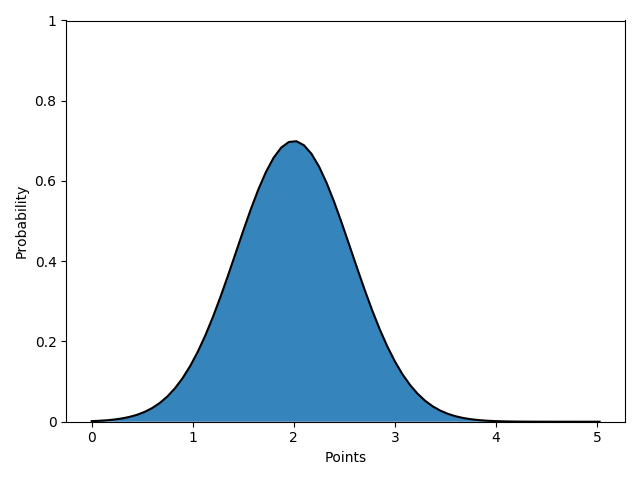
\includegraphics[width=.5\textwidth]{../assets/brier_plot.png}
		\caption{A Brier score of 0.14 expressed as a probability function over a task that would give 0 to 5 points with the correct answer at 2.}
	\end{figure}
	
	This is in comparison to what we find in the literature. In the existing studies, researchers show that humans are quite bad when self-assessing their performance after executing task. We do not know why this discrepancy exists and would like to see some further research in this field that trail possible biases by executing controlled studies. Assigning the occurring event a probability of 50\%, would be at least result in a Brier score of $BS = 0.25$. Allocating the same probability for all possible events always results in a Brier score of $BS \approx 0.84$.
	\\\\
	In future research we would like to administer a study with more subjects, find a not so homogeneous group (we only administered white German people, mainly from university).
	
	
	
	
\end{document}